\documentclass[12pt,fleqn]{article}
\usepackage[margin=1in,top=1in,bottom=1in]{geometry}
\usepackage{mathtools}
\usepackage{longtable}
\usepackage{enumitem}
\usepackage{hyperref}
\usepackage[dvips]{graphics}
\usepackage[table]{xcolor}
\usepackage{amssymb}
%\usepackage{subfig}
\usepackage{booktabs}
\usepackage{tikz}
\usepackage{subcaption}

\usepackage[normalem]{ulem}

\usepackage{multicol}
\usepackage{txfonts}
%\usepackage{amsfonts}
\usepackage{natbib}

\usepackage{wrapfig}

\usepackage{gb4e}
%\usepackage{/Users/judith/Library/Latex/drs}
%\usepackage{/Users/judith/Library/Latex/avm}
\usepackage[all]{xy}
\usepackage{rotating}
\usepackage{tipa}
\usepackage{multirow}
\usepackage{authblk}
\usepackage{adjustbox}
\usepackage{array}

\usepackage{titlesec}
\titleformat*{\section}{\bfseries\footnotesize}
 
\setlength{\parindent}{.3cm}
\setlength{\parskip}{0ex}

\setlength{\bibsep}{0mm}
\bibpunct[:]{(}{)}{;}{a}{,}{,}


\newcommand{\yi}{\'{\symbol{16}}}
\newcommand{\nasi}{\~{\symbol{16}}}
\newcommand{\hina}{h\nasi na}
\newcommand{\ina}{\nasi na}

\exewidth{(\thexnumi)}


\setlength{\bibhang}{0.5in}
\setlength{\bibsep}{0mm}
\bibpunct[:]{(}{)}{,}{a}{}{,}

\newcommand{\citepos}[1]{\citeauthor{#1}'s \citeyear{#1}}

\newcommand{\6}{\mbox{$[\hspace*{-.6mm}[$}} 
\newcommand{\9}{\mbox{$]\hspace*{-.6mm}]$}}
\newcommand{\sem}[2]{\6#1\9$^{#2}$}
\renewcommand{\ni}{\~{\i}}

\newcommand{\jt}[1]{\textbf{\color{blue}JT: #1}}


\setlength{\belowcaptionskip}{-10pt}


 \begin{document}
 
%The main text should be at most 2 pages (US Letter or A4) in length, including examples, with an optional 3rd page for references or also large graphs, tables, pictures and figures.
 
\begin{center}
{\bf Title}

Judith Degen (Stanford U) \& Judith Tonhauser (OSU / Stuttgart U)
\end{center}

\vspace*{-.2cm}

\noindent
Projection analyses have largely limited their attention to `factive' predicates, like {\em know} and {\em discover}, to the exclusion of `non-factive' ones, like {\em think} and {\em announce} (see, e.g., \citealt{heim83,vds92,abrusan2011,abrusan2016,romoli2015} and \citealt{best-question}). This limitation is motiva-

\begin{wrapfigure}{r}{0.32\textwidth}
\centering
  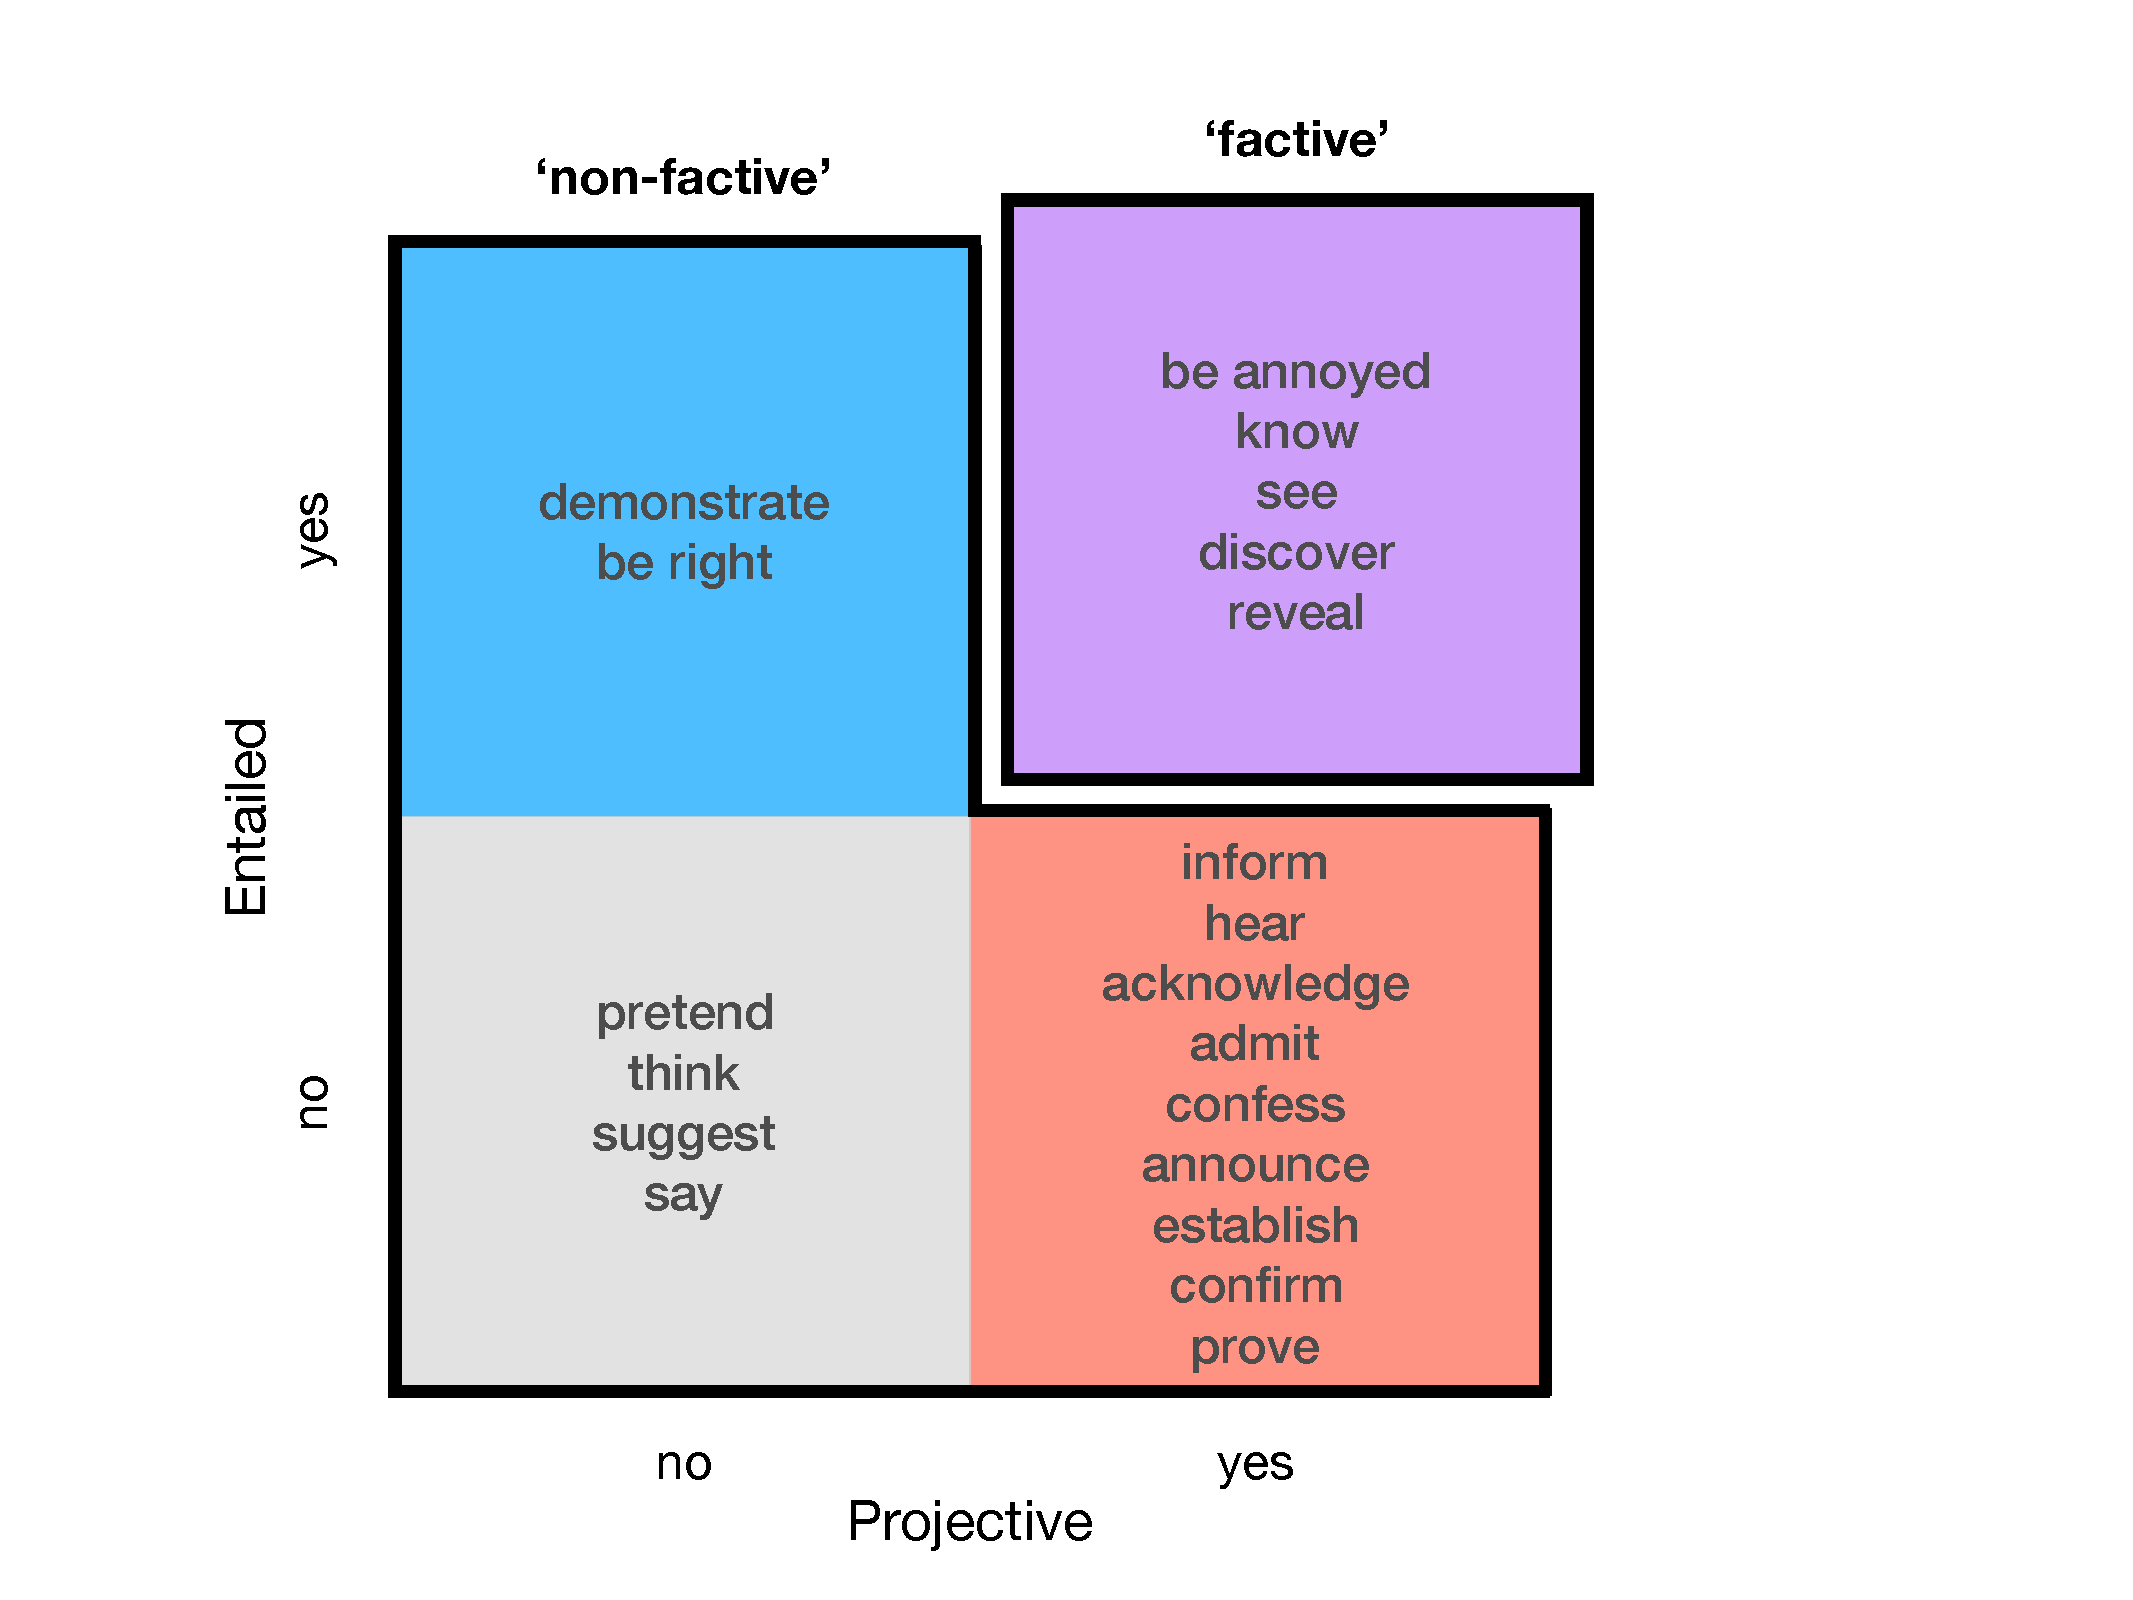
\includegraphics[trim={3.5cm 1cm 7cm 2cm},clip,width=.27\paperwidth]{../paper/figures/categorization}
  \caption{Standard classification of 20 English predicates}\label{f-cat}
\end{wrapfigure} 

\noindent
ted by the long-standing and widely-assumed assumption that `factive' predicates are empirically distinguished from `non-factive' ones (see, e.g.,\citealt{karttunen71b,kiparsky-kiparsky71} and much literature thereafter):  as shown in Fig.\ \ref{f-cat}, the content of the complement of a `factive' predicate is taken to be both projective and entailed, whereas it is not both projective and entailed for a `non-factive' one (e.g., \citealt{gazdar79a}, \citealt{ccmg90}, \citealt{vds92},  \citealt{schlenker10}, \citealt{anand-hacquard2014}, \citealt{spector-egre2015}). 

This paper investigates the empirical support for the distinction between `factive' and `non-factive' predicates by measuring projectivity and entailment for the complements of the 20 predicates in Fig.\ \ref{f-cat}. Projectivity was measured with the `certain that' diagnostic: following \citealt*{tbd-variability}, we assume that projectivity is a gradient property of content. For entailment, we applied two standard diagnostics: under the `inference' diagnostic, $p$ entails $q$ iff $q$ follows from the truth of $p$; under the `contradictoriness' diagnostic, $p$ entails $q$ iff $p$ {\em but not} $q$ is contradictory. As shown in Fig.\ \ref{f-summary-categorical}, the content of the complement of `factive' predicates (given in purple) is overall more projective than that of `non-factive' ones. However, the content of the complement of many `non-factive' predicates is projective, too. We argue that these contents constitute an exciting challenge for future projection analyses. Furthermore, we found that the entailment diagnostics do not both support an analysis of the content of the complement of the `factive' predicates as entailed; neither diagnostic provides such support for {\em reveal}. We suggest that research on entailment needs to take the pragmatics of entailment judgments more seriously (see also \citealt{demarneffe-etal2012}). {\bf BUT WHAT DO WE CONCLUDE ABOUT FACTIVE PREDS?} 

\begin{figure}[h]

\begin{subfigure}{.5\textwidth}
\centering
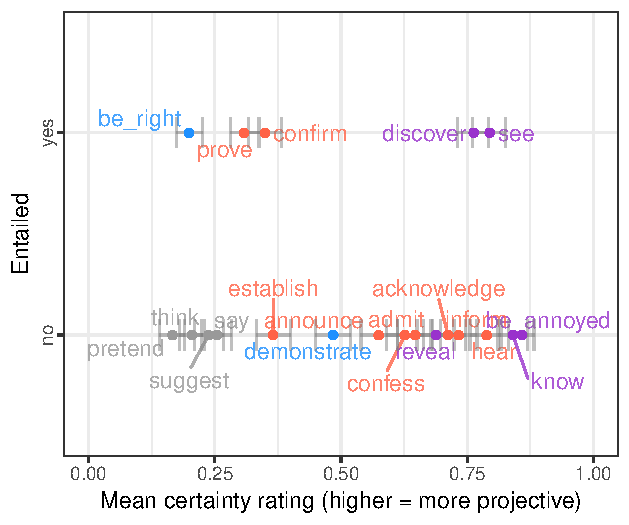
\includegraphics[width=.3\paperwidth]{../results/5-projectivity-no-fact/graphs/projection-by-inferenceEntailment}
\caption{Inference diagnostic for entailment}
\end{subfigure}%
\begin{subfigure}{.5\textwidth}
\centering
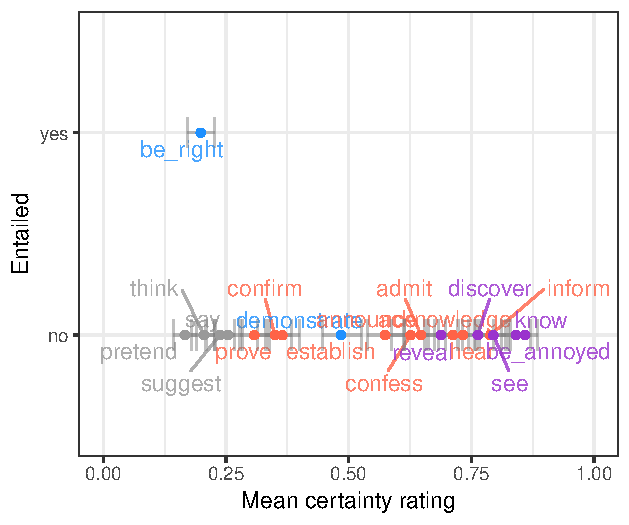
\includegraphics[width=.3\paperwidth]{../results/5-projectivity-no-fact/graphs/projection-by-contradictorinessEntailment}
\caption{Contradictoriness diagnostic for entailment}
\end{subfigure}

\caption{Mean certainty rating (with 95\% CIs) of the content of the complement of 20 predicates by whether the content is entailed under the (a) inference or (b) contradictoriness diagnostic.}\label{f-summary-categorical}

\end{figure}

\newpage

\bibliographystyle{/Users/tonhauser.1/Library/Latex/cslipubs-natbib}
\bibliography{/Users/tonhauser.1/Documents/bibliography}

\end{document}
